\documentclass[11pt,letterpaper]{article}
\usepackage[margin=1.0in]{geometry}
\usepackage[utf8]{inputenc}
\usepackage{cite}
\usepackage{amsmath}
\usepackage{amsfonts}
\usepackage{amssymb}
\usepackage{makeidx}
\usepackage{graphicx}
\setlength\parindent{0pt}

\author{STUDENT XXXX}
\title{HW: Time of Flight Measurement}

\begin{document}

\maketitle

The Time of Flight principle essentially uses the time that passes between two (or more) events to deduce information from a system. For example when we use ultrasonic sensing, we generate a pulse, and wait until we sense a reflected pulse from an object. Then we use the time difference, combined with a known speed of sound at a certain temperature to determine the distance from the sensor to the object. Modern Light Detection and Ranging (LIDAR) devices do the same thing using the speed of light.\\ 

Figure \ref{fig:HW_TimeOfFlightMeasurement1} shows an example of a Time of Flight device that was developed to measure the diameter and velocity of granular fertilizer particles. One of the complications was that the measurement sensors consisted of 5 mm wide OptoSchmitt sensors, which would make it impossible to detect a 1 mm particle. Therefore the shadow of the particles was magnified using two lenses as in a slide projector. By magnifying the image of the particles in real time (this is the beauty of using optical detection, the speed of light is approx. 300,000 km/s) it was possible to reliably detect particles with a size of 1 mm.\\  

\begin{figure}
\centering
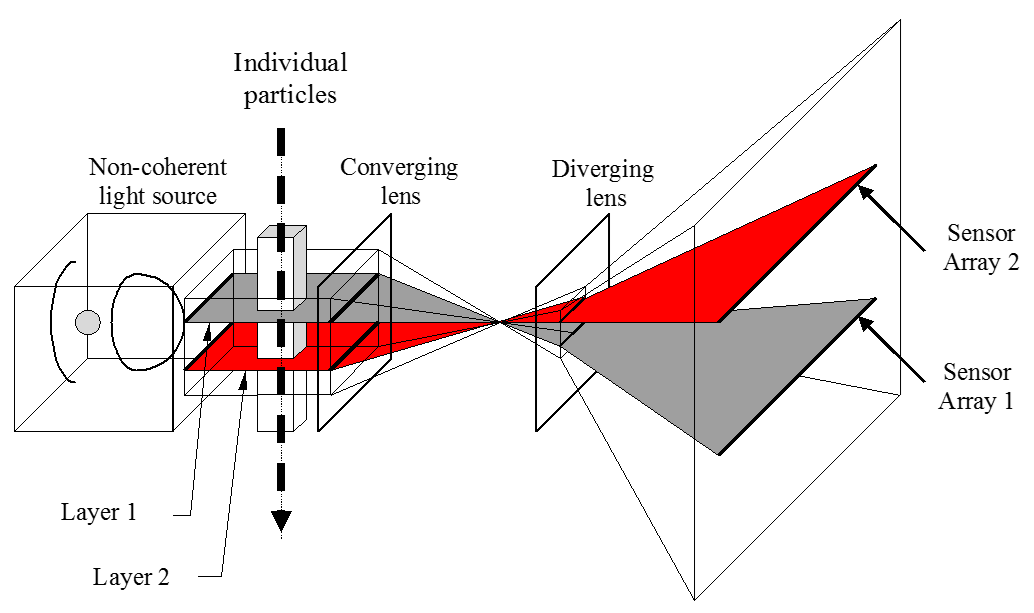
\includegraphics[width=0.65\linewidth]{HW_TimeOfFlightMeasurement1}
\caption{Optical Time of Flight sensor that was used to measure the velocity and diameter of individual fertilizer particles with a diameter ranging from 1-5 mm. Since the sensor array consisted of relatively large sensors (SDP8600 OptoSchmitt's) with a width of 5mm, optical magnification (as in a slide projector) was applied.}
\label{fig:HW_TimeOfFlightMeasurement1}
\end{figure}

To analyze the working of the sensor, imagine that the round object on the left is moving upward at a constant velocity (Figure \ref{fig:HW_TimeOfFlightMeasurement2}) while interrupting the dual optical detection layers. The graph shows the distance as a function of time, as a straight line, which implies that the velocity is constant, rendering the acceleration equal to zero. Under the assumption of a constant velocity, the time it takes an object to move through the distance b from layer 1 to layer 2 is $\Delta t_f$. Therefore the velocity $v_0$ is simply:

\begin{figure}
\centering
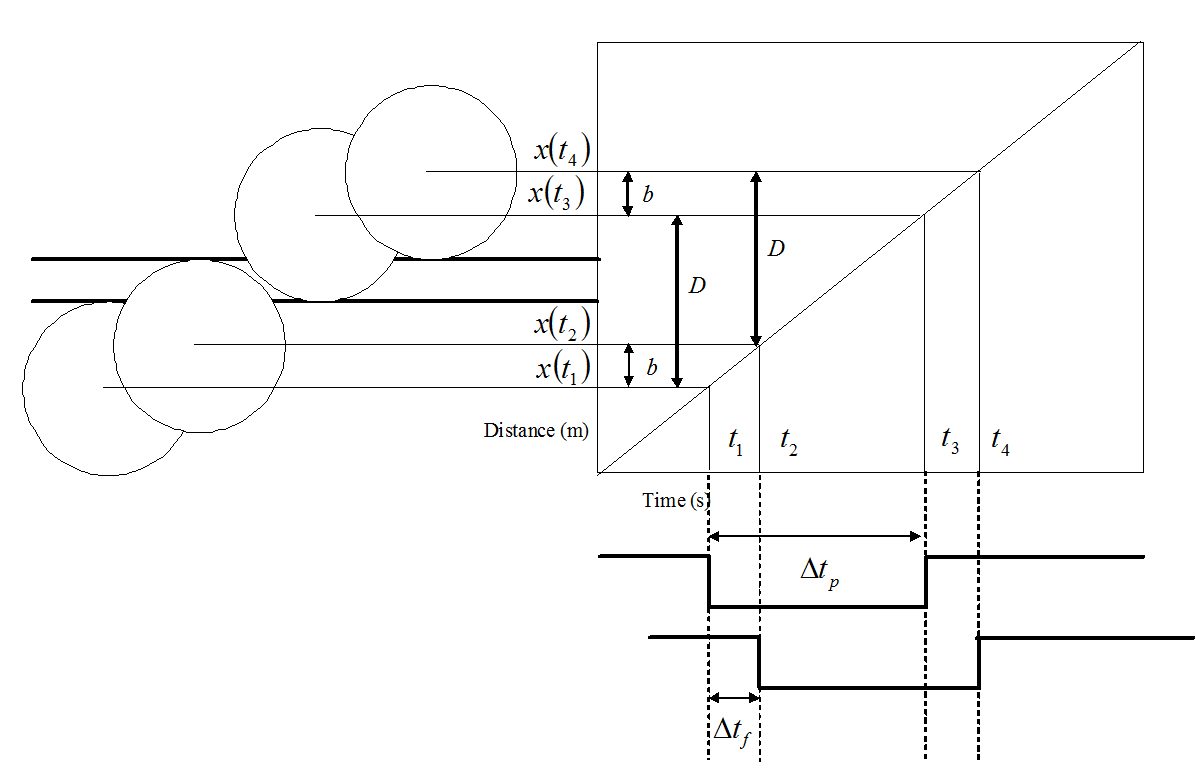
\includegraphics[width=0.9\linewidth]{HW_TimeOfFlightMeasurement2}
\caption{Relationship between interruption events in space (left) and associated interruption events in time (bottom). The fact that the relationship between distance and time can be captured using a straight line indicates that the velocity of the objects must be constant.}
\label{fig:HW_TimeOfFlightMeasurement2}
\end{figure}

\begin{equation} \label{Eqn:HW_TimeOfFlightMeasurement1}
v_0 = \dfrac{b}{\Delta t_f}
\end{equation}

The diameter of the object is represented by the time it takes to move the object through one of the light layers times the velocity of the object or:

\begin{equation} \label{Eqn:HW_TimeOfFlightMeasurement2}
D = v \Delta t_p = b \dfrac{\Delta t_p}{\Delta t_f}
\end{equation}

These relationships are easy to see in the case of a constant velocity, which implies zero acceleration. However, if there is a constant acceleration, it is not that obvious anymore, and we need to use proper analysis to find out how the dimensions of our object are related to the times measured. First, let's propose a (correct) equation that relates distance to time for the constant velocity case:

\begin{equation} \label{Eqn:HW_TimeOfFlightMeasurement3}
x(t) = x_0 + v_0t
\end{equation}

To determine how our constant velocity $v_0$ is related to the timing information, we can construct a relationship graph as shown in Figure \ref{fig:HW_TimeOfFlightMeasurement2}. We know two measures 1) that the distance to move the particle from $x(t_1)$ to $x(t_2)$ is equal to $b$ and 2) that the time associated with that movement is $\Delta t_f$. We also know that the the distance from $x(t_1)$ to $x(t_3)$ is equal to $D$, which is the diameter (major axis) of our particles and that the time associated with this movement is $\Delta t_p$. We will use both these to determine the general equations to measure the velocity $v_0$ and the particle diameter $D$ as follows: 

\begin{align}\label{Eqn:HW_TimeOfFlightMeasurement4}
&x(t_1) = v_0 t_1 + x_0 \\
&x(t_2) = v_0 t_2 + x_0 \\
&x(t_2) - x(t_1) = b = (v_0 t_2 + x_0) - (v_0 t_1 + x_0) = v_0 (t_2 - t_1) = v_0 \Delta t_f\\
&b = v_0 \Delta t_f\\
&v_0 = \dfrac{b}{\Delta t_f}
\end{align}

\begin{align}\label{Eqn:HW_TimeOfFlightMeasurement5}
&x(t_3) = v_0 t_3 + x_0 \\
&x(t_1) = v_0 t_1 + x_0 \\
&x(t_3) - x(t_1) = D = (v_0 t_3 + x_0) - (v_0 t_1 + x_0) = v_0 (t_3 - t_1) = v_0 \Delta t_p\\
&D = v_0 \Delta t_p\\
&D = \dfrac{b}{\Delta t_f} \Delta t_p = b \dfrac{\Delta t_p}{\Delta t_f}
\end{align}

Figure \ref{fig:HW_TimeOfFlightMeasurement3} shows the situation for an object with constant diameter moving at a constant acceleration. 

\begin{figure}
\centering
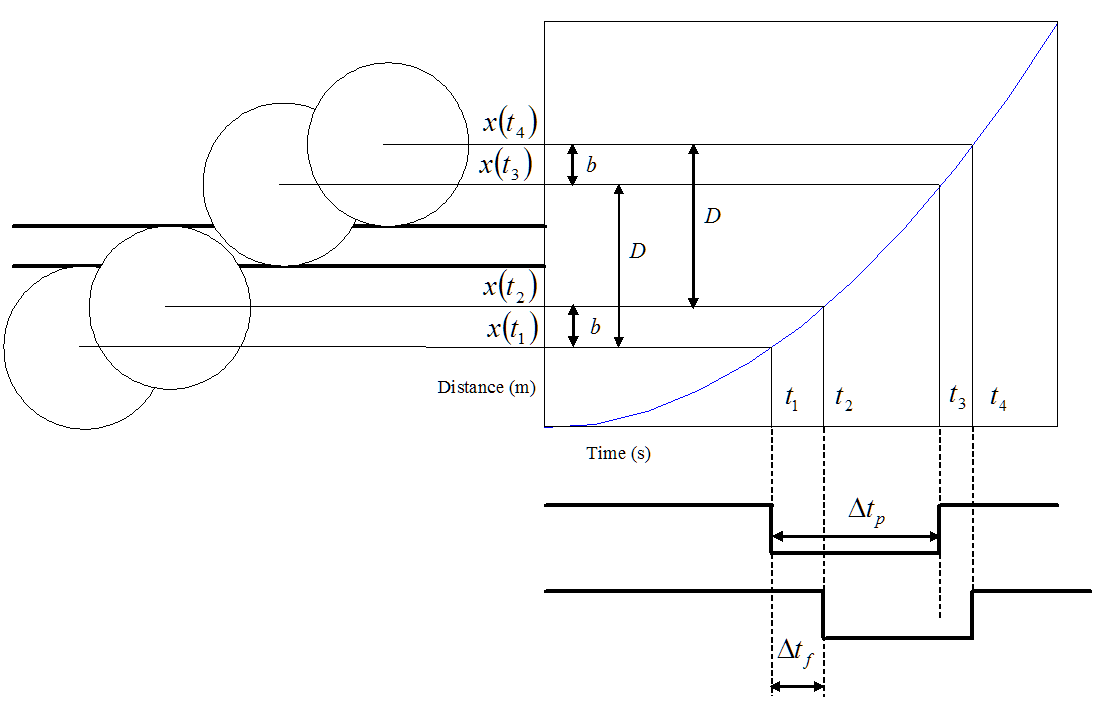
\includegraphics[width=0.8\linewidth]{HW_TimeOfFlightMeasurement3}
\caption{Relationship between interruption events (left) and associated photo-interruption events (bottom). Here the assumption is made that the velocity of the particles is not constant, but that they have a constant acceleration $a$.}
\label{fig:HW_TimeOfFlightMeasurement3}
\end{figure}

Using the same methodology as shown for the constant velocity case, your job is to derive the equation for the Diameter of the particle as a function of the acceleration $a$, the distance between the sensor layers $b$ as well as $\Delta t_f$ and $\Delta t_p$. This means that the general equation of motion becomes:

\begin{equation} \label{Eqn:HW_TimeOfFlightMeasurement6}
x(t) = x_0 + v_0t +\dfrac{1}{2}at^2
\end{equation}

Where $a$ is a constant acceleration in $ms^{-2}$. You do not need to solve for the acceleration $a$, you can leave it in the final equation for the diameter.

\begin{equation} \label{Eqn:HW_TimeOfFlightMeasurement7}
D=f(a,b,\Delta t_f, \Delta t_p)
\end{equation}

\textbf{Use LaTex functionality, so just continue this document, and extend it to include your answer. Submit the pdf file of this document and don't forget to put your name at the top.}

\end{document}